\documentclass[11pt,a4paper]{article}
\usepackage[utf8]{inputenc}
\usepackage[margin=2.3cm]{geometry}
\usepackage{amsmath,amssymb,amsfonts,amsthm}
\usepackage{tcolorbox}
\tcbuselibrary{skins,breakable}
\usepackage{tikz}
\usetikzlibrary{shapes.geometric,arrows.meta,positioning,calc,decorations.pathreplacing}
\usepackage{booktabs}
\usepackage{tabularx}
\usepackage{circuitikz}
\usepackage{enumitem}
\usepackage{listings}
\usepackage{hyperref}

\hypersetup{
    colorlinks=true,
    linkcolor=headercolor,
    citecolor=headercolor,
    urlcolor=blue!70!black,
    pdfauthor={Ir. Novalio Daratha, S.T., M.Sc., Ph.D. and Muhammad Arfan, S.T., M.T.},
    pdftitle={Modul 15: Polinomial Legendre, Koordinat Bola, dan 4 Persamaan Maxwell Diferensial}
}

% Palet Warna Institusional
\definecolor{headercolor}{RGB}{0, 32, 96}     % Biru Navy UNIB
\definecolor{accentcolor}{RGB}{197, 160, 89}   % Emas / Gold UNIB
\definecolor{softgreen}{RGB}{235, 247, 238}    % Latar Hijau Lembut
\definecolor{darkgreen}{RGB}{34, 112, 60}     % Aksen Hijau
\definecolor{softblue}{RGB}{240, 244, 250}     % Latar Biru Lembut
\definecolor{softgray}{RGB}{248, 249, 250}     % Latar Abu-abu Lembut
\definecolor{darkgray}{RGB}{60, 64, 67}       % Teks Abu-abu

% Konfigurasi Kotak OBE & Teorema
\newtcolorbox{subcpmkbox}{
    colback=softblue,
    colframe=headercolor,
    fonttitle=\bfseries\color{white},
    title={Capaian Pembelajaran Modul (Sub-CPMK 15 -- OBE Framework)},
    arc=4pt,
    left=12pt, right=12pt, top=10pt, bottom=10pt,
    boxrule=1.2pt
}

\newtcolorbox{theorembox}[1]{
    colback=softgreen,
    colframe=darkgreen,
    fonttitle=\bfseries\color{white},
    title={#1},
    arc=3pt,
    left=10pt, right=10pt, top=8pt, bottom=8pt,
    boxrule=1pt
}

\newtcolorbox{casebox}[1]{
    colback=white,
    colframe=headercolor,
    fonttitle=\bfseries\color{white},
    title={Studi Kasus Industri: #1},
    arc=3pt,
    left=10pt, right=10pt, top=8pt, bottom=8pt,
    boxrule=1pt
}

\newtcolorbox{tipbox}{
    colback=softgray,
    colframe=accentcolor,
    fonttitle=\bfseries\color{headercolor},
    title={Wawasan Fisika \& Rekayasa Elektro},
    arc=3pt,
    left=10pt, right=10pt, top=8pt, bottom=8pt,
    boxrule=1pt
}

\theoremstyle{definition}
\newtheorem{example}{Contoh Soal}[section]

% Format Listing Julia
\lstdefinelanguage{Julia}%
  {morekeywords={abstract,break,case,catch,const,continue,do,else,elseif,%
      end,export,false,for,function,immutable,import,importall,if,in,%
      macro,module,quote,return,true,try,type,typealias,using,while},%
   sensitive=true,%
   morecomment=[l]{\#},%
   morecomment=[n]{\#=}{=\#},%
   morestring=[b]',%
   morestring=[m]"%
  }[keywords,comments,strings]

\lstset{
    language=Julia,
    basicstyle=\ttfamily\footnotesize,
    keywordstyle=\bfseries\color{headercolor},
    commentstyle=\color{gray}\itshape,
    stringstyle=\color{darkgreen},
    backgroundcolor=\color{softgray},
    frame=single,
    rulecolor=\color{lightgray},
    breaklines=true,
    breakatwhitespace=true,
    showstringspaces=false,
    tabsize=4,
    xleftmargin=12pt,
    xrightmargin=12pt
}

\title{
    \vspace{-1.2cm}
    \textbf{\Large MODUL AJAR KULIAH MINGGU 15}\\[0.25cm]
    \textbf{\LARGE POLINOMIAL LEGENDRE, KOORDINAT BOLA, DAN 4 PERSAMAAN MAXWELL DIFERENSIAL}\\[0.2cm]
    \large Solusi Potensial Bola, Arus Pergeseran, Gelombang Elektromagnetik, dan Sintesis Kurikulum Persamaan Diferensial Rekayasa Elektro
}
\author{
    \textbf{Ir. Novalio Daratha, S.T., M.Sc., Ph.D.} \& \textbf{Muhammad Arfan, S.T., M.T.}\\
    Jurusan Teknik Elektro -- Fakultas Teknik, Universitas Bengkulu\\
    \texttt{\{novalio, arfan\}@unib.ac.id}
}
\date{Pekan Perkuliahan ke-15 -- Semester Genap 2026}

\begin{document}

\maketitle

\begin{abstract}
Modul ke-15 ini merupakan puncak integratif dari seluruh rangkaian perkuliahan Persamaan Diferensial dalam kurikulum S1 Teknik Elektro. Modul ini menyatukan dua fondasi matematika tingkat tinggi: solusi persamaan potensial Laplace dalam koordinat bola $(r, \theta, \phi)$ melalui metode pemisahan variabel yang melahirkan Persamaan Diferensial Legendre dan Polinomial Legendre $P_n(\cos\theta)$, serta formulasi diferensial dari 4 Persamaan Maxwell (Hukum Gauss Listrik, Hukum Gauss Magnetik, Hukum Induksi Faraday, dan Hukum Ampere-Maxwell). Mahasiswa dibimbing untuk menurunkan secara eksklusif dari prinsip pertama (\textit{first principles}) persamaan gelombang medan elektromagnetik skalar dan vektor ($\nabla^2 \vec{E} - \mu_0\epsilon_0 \frac{\partial^2 \vec{E}}{\partial t^2} = 0$), mengungkap makna fisis arus pergeseran (\textit{displacement current}), serta mengevaluasi medan listrik di sekitar bola konduktor netral dan pembumian gardu induk berdasarkan standar IEEE Std 605 dan IEC 62271. Modul dilengkapi dengan komputasi ilmiah terbuka berbasis bahasa Julia, bank soal bertingkat taksonomi Bloom C1 hingga C6, serta matriks sintesis komprehensif penutup yang menghubungkan PDB orde 1, PDB orde 2, Transformasi Laplace, Deret Fourier, dan PDP menuju penguasaan medan elektromagnetika lanjut.
\end{abstract}

\vspace{0.2cm}

\begin{subcpmkbox}
Setelah menuntaskan pembelajaran pada Modul Minggu ke-15 ini, mahasiswa diharapkan mampu:
\begin{enumerate}[leftmargin=*]
    \item \textbf{C1 (Mengingat):} Menyebutkan bentuk diferensial dan integral dari 4 Persamaan Maxwell serta mengenali bentuk standar Persamaan Diferensial Legendre.
    \item \textbf{C2 (Memahami):} Menjelaskan peran fisis arus pergeseran Maxwell $\partial \vec{D}/\partial t$ dalam menjaga kekekalan muatan kontinuitas listrik dan prinsip ortogonalitas Polinomial Legendre $P_n(x)$.
    \item \textbf{C3 (Menerapkan):} Menurunkan solusi potensial elektrostatik $V(r, \theta)$ di dalam dan di luar bola konduktor berjari-jari $a$ yang ditempatkan dalam medan listrik seragam eksternal $E_0 \hat{a}_z$.
    \item \textbf{C4 (Menganalisis):} Menurunkan persamaan gelombang elektromagnetik dari Persamaan Maxwell dan membuktikan bahwa kecepatan rambat gelombang transversal dalam ruang hampa tepat bernilai $c = 1/\sqrt{\mu_0 \epsilon_0} \approx 3 \times 10^8\text{ m/s}$.
    \item \textbf{C5 (Mengevaluasi):} Memvalidasi kesamaan nilai arus konduksi $I_c$ pada kawat penghantar dan arus pergeseran $I_d$ di dalam celah isolator dielektrik kapasitor pelat sejajar berfrekuensi tinggi.
    \item \textbf{C6 (Merancang \& Menyintesis):} Menyintesis peta konseptual menyeluruh yang menghubungkan pemodelan rangkaian listrik terpusat (PDB orde 1 \& 2), analisis domain frekuensi kompleks (Laplace), representasi harmonisa (Fourier), dan persamaan medan terdistribusi (PDP) sebagai fondasi rekayasa elektro modern.
\end{enumerate}
\end{subcpmkbox}

\section{Peta Konsep \& Kedudukan Modul dalam Kurikulum}

Modul Minggu ke-15 menandai garis finis materi perkuliahan Persamaan Diferensial sebelum pelaksanaan Ujian Akhir Semester (UAS). Jika Modul 1 sampai 7 memfokuskan kajian pada rangkaian listrik parameter terpusat (\textit{lumped parameters}) yang dimodelkan oleh PDB dan Transformasi Laplace, dan Modul 9 sampai 14 menguraikan sistem terdistribusi (\textit{distributed parameters}) melalui PDP Gelombang 1D, Panas 1D, Laplace 2D Kartesian, dan Bessel Silindris, maka Modul 15 ini merupakan sintesis unifikasi terbesar: menyelesaikan geometri bola 3D dengan Polinomial Legendre dan merangkum seluruh hukum kelistrikan dan kemagnetan ke dalam 4 Persamaan Diferensial Maxwell.

Posisi strategis Modul Minggu 15 disajikan pada Gambar~\ref{fig:peta_jalan_pd_w15}.

\begin{figure}[htbp]
\centering
\resizebox{\linewidth}{!}{%
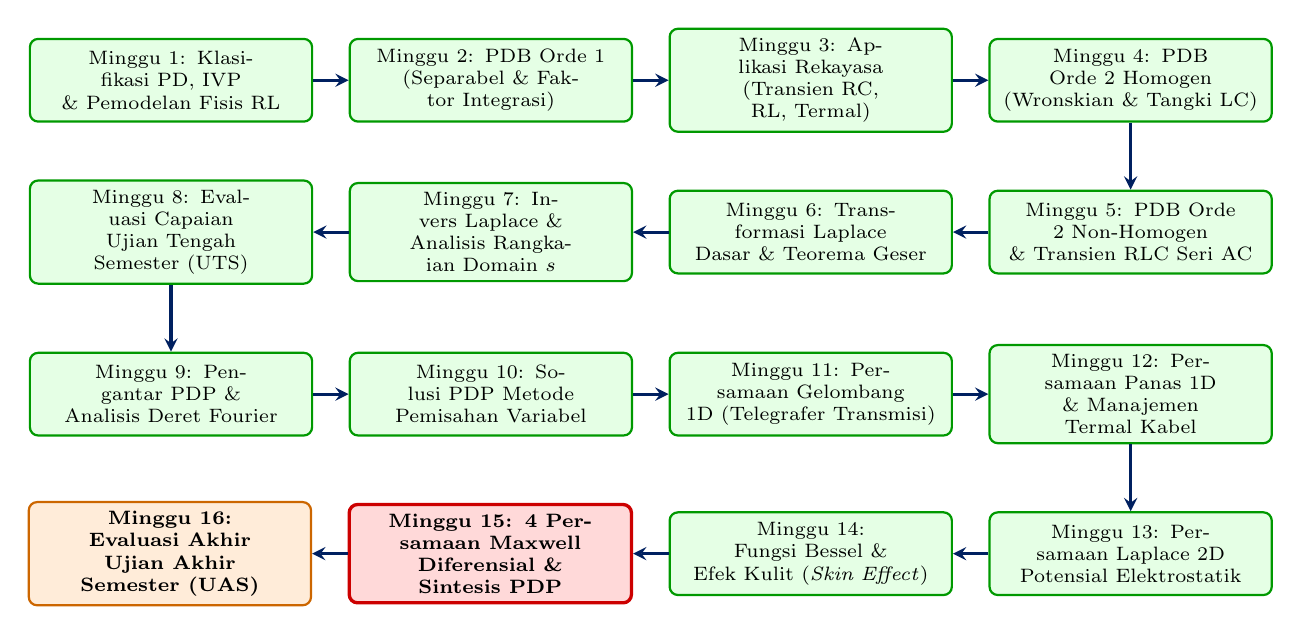
\begin{tikzpicture}[
    node distance=0.85cm and 0.45cm,
    block/.style={rectangle, draw=headercolor, fill=blue!8, thick, rounded corners=3pt, align=center, text width=3.35cm, minimum height=1.05cm, font=\scriptsize},
    doneblock/.style={rectangle, draw=green!60!black, fill=green!10, thick, rounded corners=3pt, align=center, text width=3.35cm, minimum height=1.05cm, font=\scriptsize},
    highlight/.style={rectangle, draw=red!80!black, fill=red!15, very thick, rounded corners=3pt, align=center, text width=3.35cm, minimum height=1.05cm, font=\scriptsize\bfseries},
    midblock/.style={rectangle, draw=orange!80!black, fill=orange!15, thick, rounded corners=3pt, align=center, text width=3.35cm, minimum height=1.05cm, font=\scriptsize\bfseries},
    arrow/.style={->, >=stealth, line width=1.1pt, headercolor}
]
    % Paruh 1: PDB & Rangkaian Listrik
    \node[doneblock] (w1) {Minggu 1: Klasifikasi PD, IVP\\\& Pemodelan Fisis RL};
    \node[doneblock, right=of w1] (w2) {Minggu 2: PDB Orde 1\\(Separabel \& Faktor Integrasi)};
    \node[doneblock, right=of w2] (w3) {Minggu 3: Aplikasi Rekayasa\\(Transien RC, RL, Termal)};
    \node[doneblock, right=of w3] (w4) {Minggu 4: PDB Orde 2 Homogen\\(Wronskian \& Tangki LC)};
    
    \node[doneblock, below=of w4] (w5) {Minggu 5: PDB Orde 2 Non-Homogen\\\& Transien RLC Seri AC};
    \node[doneblock, left=of w5] (w6) {Minggu 6: Transformasi Laplace\\Dasar \& Teorema Geser};
    \node[doneblock, left=of w6] (w7) {Minggu 7: Invers Laplace \&\\Analisis Rangkaian Domain $s$};
    \node[doneblock, left=of w7] (w8) {Minggu 8: Evaluasi Capaian\\Ujian Tengah Semester (UTS)};
    
    % Paruh 2: PDP & Medan Elektromagnetika
    \node[doneblock, below=of w8] (w9) {Minggu 9: Pengantar PDP \&\\Analisis Deret Fourier};
    \node[doneblock, right=of w9] (w10) {Minggu 10: Solusi PDP Metode\\Pemisahan Variabel};
    \node[doneblock, right=of w10] (w11) {Minggu 11: Persamaan Gelombang\\1D (Telegrafer Transmisi)};
    \node[doneblock, right=of w11] (w12) {Minggu 12: Persamaan Panas 1D\\\& Manajemen Termal Kabel};
    
    \node[doneblock, below=of w12] (w13) {Minggu 13: Persamaan Laplace 2D\\Potensial Elektrostatik};
    \node[doneblock, left=of w13] (w14) {Minggu 14: Fungsi Bessel \&\\Efek Kulit (\textit{Skin Effect})};
    \node[highlight, left=of w14] (w15) {Minggu 15: 4 Persamaan Maxwell\\Diferensial \& Sintesis PDP};
    \node[midblock, left=of w15] (w16) {Minggu 16: Evaluasi Akhir\\Ujian Akhir Semester (UAS)};
    
    \draw[arrow] (w1) -- (w2);
    \draw[arrow] (w2) -- (w3);
    \draw[arrow] (w3) -- (w4);
    \draw[arrow] (w4) -- (w5);
    \draw[arrow] (w5) -- (w6);
    \draw[arrow] (w6) -- (w7);
    \draw[arrow] (w7) -- (w8);
    \draw[arrow] (w8) -- (w9);
    \draw[arrow] (w9) -- (w10);
    \draw[arrow] (w10) -- (w11);
    \draw[arrow] (w11) -- (w12);
    \draw[arrow] (w12) -- (w13);
    \draw[arrow] (w13) -- (w14);
    \draw[arrow] (w14) -- (w15);
    \draw[arrow] (w15) -- (w16);
\end{tikzpicture}%
}
\caption{Peta jalan kurikulum perkuliahan dengan penekanan pada Modul Penutup Minggu 15.}
\label{fig:peta_jalan_pd_w15}
\end{figure}

\section{Pendahuluan \& Filosofi Fisika: Puncak Unifikasi Elektromagnetika}

Sepanjang sejarah sains dan rekayasa, salah satu pencapaian intelektual terbesar umat manusia terjadi pada pertengahan abad ke-19 ketika fisikawan dan matematikawan Skotlandia, James Clerk Maxwell, berhasil merumuskan sintesis matematis komprehensif yang menyatukan kelistrikan, kemagnetan, dan optika ke dalam satu kerangka kerja teoretis tunggal. 

Sebelum Maxwell, para insinyur dan ilmuwan memperlakukan medan listrik (yang dijelaskan oleh Coulomb dan Gauss), medan magnetik (yang dijelaskan oleh Biot-Savart dan Ampere), serta gaya gerak listrik induksi (yang ditemukan oleh Faraday) sebagai fenomena alam yang terpisah-pisah. Melalui ketajaman kalkulus diferensial dan vektor, Maxwell menyadari bahwa Hukum Ampere yang ada saat itu secara matematis tidak konsisten dengan hukum kekekalan muatan listrik ketika diterapkan pada arus bolak-balik berfrekuensi tinggi. 

Dengan menambahkan satu suku koreksi matematis yang revolusioner—dikenal sebagai \textbf{Arus Pergeseran} (\textit{Displacement Current}) $\frac{\partial \vec{D}}{\partial t}$—Maxwell tidak hanya menutup inkonsistensi kalkulus tersebut, tetapi juga secara tak terduga menurunkan persamaan diferensial parsial orde dua hiperbolik: \textbf{Persamaan Gelombang Elektromagnetik}. Kecepatan rambat gelombang yang diprediksi oleh persamaan diferensial ini ternyata bertepatan persis dengan kecepatan cahaya yang telah diukur di laboratorium:
\begin{equation}
    c = \frac{1}{\sqrt{\mu_0 \epsilon_0}} \approx 2{,}99792 \times 10^8\text{ m/s}
\end{equation}
Kesimpulan filosofisnya sangat menakjubkan: \textit{cahaya tampak, gelombang radio, sinar ultraviolet, dan gelombang mikro sesungguhnya adalah perambatan gelombang diferensial medan elektromagnetik yang saling menginduksi di ruang hampa}.

Di sisi lain, untuk menganalisis distribusi medan dan potensial elektrostatik pada geometri bola—seperti bola elektroda penangkal petir, bola pembumian gardu induk (\textit{grounding sphere}), isolator tegangan tinggi keramik berbentuk bola, dan tetesan air pada kawat fasa SUTET—persamaan Laplace dalam koordinat bola melahirkan fungsi ortogonal kedua yang sangat penting: \textbf{Polinomial Legendre}. Modul 15 ini menuntaskan pembahasan kedua topik monumental tersebut.

\section{Koordinat Bola, Pemisahan Variabel, dan Persamaan Legendre}

\subsection{Persamaan Laplace dalam Koordinat Bola}
Dalam sistem koordinat bola $(r, \theta, \phi)$, di mana $r \ge 0$ adalah jari-jari radial, $0 \le \theta \le \pi$ adalah sudut zenit/kutub (\textit{colatitude}), dan $0 \le \phi < 2\pi$ adalah sudut azimut, operator Laplacian $\nabla^2 V$ didefinisikan secara lengkap sebagai:
\begin{equation}
    \nabla^2 V = \frac{1}{r^2} \frac{\partial}{\partial r}\left( r^2 \frac{\partial V}{\partial r} \right) + \frac{1}{r^2 \sin\theta} \frac{\partial}{\partial \theta}\left( \sin\theta \frac{\partial V}{\partial \theta} \right) + \frac{1}{r^2 \sin^2\theta} \frac{\partial^2 V}{\partial \phi^2} = 0
    \label{eq:laplace_spherical}
\end{equation}

Dalam sebagian besar aplikasi rekayasa elektro tenaga (seperti bola elektroda dalam medan listrik aksial seragam), sistem memiliki \textbf{simetri azimut}, yang berarti potensial tidak bergantung pada sudut rotasi $\phi$ ($\partial V/\partial \phi = 0$). Dengan asumsi simetri azimut ini, Persamaan~\eqref{eq:laplace_spherical} tereduksi menjadi:
\begin{equation}
    \frac{\partial}{\partial r}\left( r^2 \frac{\partial V}{\partial r} \right) + \frac{1}{\sin\theta} \frac{\partial}{\partial \theta}\left( \sin\theta \frac{\partial V}{\partial \theta} \right) = 0
    \label{eq:laplace_axisymmetric}
\end{equation}

\subsection{Pemisahan Variabel \& Munculnya Persamaan Legendre}
Kita terapkan metode pemisahan variabel dengan mengasumsikan solusi berbentuk perkalian fungsi radial dan fungsi sudut:
\begin{equation}
    V(r, \theta) = R(r) \, \Theta(\theta)
\end{equation}
Substitusikan bentuk ini ke dalam Persamaan~\eqref{eq:laplace_axisymmetric} dan bagi kedua ruas dengan $R(r) \Theta(\theta)$:
\begin{equation}
    \frac{1}{R(r)} \frac{d}{dr}\left( r^2 \frac{dR}{dr} \right) + \frac{1}{\Theta(\theta) \sin\theta} \frac{d}{d\theta}\left( \sin\theta \frac{d\Theta}{d\theta} \right) = 0
    \label{eq:separation_spherical}
\end{equation}
Suku pertama hanya bergantung pada $r$, sedangkan suku kedua hanya bergantung pada $\theta$. Agar jumlah keduanya selalu nol untuk setiap $r$ dan $\theta$, masing-masing suku harus bernilai konstanta pemisah. Kita pilih konstanta pemisah standar dalam mekanika dan elektromagnetika, yaitu $n(n+1)$ di mana $n$ adalah bilangan bulat non-negatif ($n = 0, 1, 2, \dots$):
\begin{align}
    \frac{d}{dr}\left( r^2 \frac{dR}{dr} \right) - n(n+1) R &= 0 \label{eq:radial_ode} \\
    \frac{1}{\sin\theta} \frac{d}{d\theta}\left( \sin\theta \frac{d\Theta}{d\theta} \right) + n(n+1) \Theta &= 0 \label{eq:angular_ode}
\end{align}

\subsection{Persamaan Diferensial Legendre}
Untuk menyelesaikan persamaan sudut~\eqref{eq:angular_ode}, kita lakukan substitusi variabel koordinat:
\begin{equation}
    x = \cos\theta \implies \frac{dx}{d\theta} = -\sin\theta, \quad \sin^2\theta = 1 - x^2
\end{equation}
Dengan menerapkan aturan rantai turunan, Persamaan~\eqref{eq:angular_ode} bertransformasi menjadi:
\begin{equation}
    (1 - x^2) \frac{d^2 \Theta}{dx^2} - 2x \frac{d\Theta}{dx} + n(n+1)\Theta = 0
    \label{eq:legendre_ode}
\end{equation}
Persamaan diferensial~\eqref{eq:legendre_ode} adalah \textbf{Persamaan Diferensial Legendre Orde $n$}.

\subsection{Polinomial Legendre \texorpdfstring{$P_n(x)$}{P\_n(x)} \& Rumus Rodrigues}
Persamaan Legendre memiliki dua solusi linier independen: $P_n(x)$ (Polinomial Legendre jenis pertama) dan $Q_n(x)$ (Fungsi Legendre jenis kedua). Namun, fungsi $Q_n(x)$ meledak menuju tak terhingga ($\pm \infty$) pada kutub utara dan kutub selatan bola ($x = \cos 0 = 1$ dan $x = \cos\pi = -1$). Karena potensial listrik fisik pada kutub bola harus selalu berhingga (\textit{physically bounded}), maka koefisien $Q_n(x)$ harus nol ($C_2 = 0$).

Solusi yang diterima secara fisik adalah \textbf{Polinomial Legendre} $P_n(x)$, yang dapat diturunkan secara eksplisit menggunakan \textbf{Rumus Rodrigues}:
\begin{equation}
    P_n(x) = \frac{1}{2^n n!} \frac{d^n}{dx^n} \left[ (x^2 - 1)^n \right]
    \label{eq:rodrigues_formula}
\end{equation}

Berikut lima Polinomial Legendre pertama yang paling sering diterapkan dalam rekayasa:
\begin{align}
    P_0(x) &= 1 \\
    P_1(x) &= x = \cos\theta \\
    P_2(x) &= \frac{1}{2}(3x^2 - 1) = \frac{1}{4}(3\cos 2\theta + 1) \\
    P_3(x) &= \frac{1}{2}(5x^3 - 3x) = \frac{1}{8}(5\cos 3\theta + 3\cos\theta) \\
    P_4(x) &= \frac{1}{8}(35x^4 - 30x^2 + 3)
\end{align}

\begin{theorembox}{Sifat Ortogonalitas Polinomial Legendre}
Polinomial Legendre membentuk himpunan fungsi basis ortogonal pada interval $x \in [-1, 1]$ (yaitu $\theta \in [0, \pi]$):
\begin{equation}
    \int_{-1}^{1} P_n(x) P_m(x) \, dx = \int_{0}^{\pi} P_n(\cos\theta) P_m(\cos\theta) \sin\theta \, d\theta = 
    \begin{cases}
        0, & \text{jika } n \neq m \\
        \dfrac{2}{2n + 1}, & \text{jika } n = m
    \end{cases}
    \label{eq:legendre_orthogonality}
\end{equation}
Sifat ortogonalitas ini memungkinkan kita mengekspansikan fungsi potensial batas arbitrer pada permukaan bola menjadi deret Fourier-Legendre.
\end{theorembox}

\subsection{Solusi Persamaan Radial \& Solusi Umum Potensial Bola}
Persamaan radial~\eqref{eq:radial_ode} adalah persamaan Cauchy-Euler:
\begin{equation}
    r^2 \frac{d^2 R}{dr^2} + 2r \frac{dR}{dr} - n(n+1) R = 0
\end{equation}
Dengan memisalkan $R(r) = r^p$, kita peroleh persamaan karakteristik:
\begin{equation}
    p(p-1) + 2p - n(n+1) = 0 \implies p^2 + p - n(n+1) = (p - n)(p + n + 1) = 0
\end{equation}
Akar-akar karakteristiknya adalah $p_1 = n$ dan $p_2 = -(n+1)$. Maka solusi umum radial adalah:
\begin{equation}
    R_n(r) = A_n r^n + \frac{B_n}{r^{n+1}}
\end{equation}
Menggabungkan solusi radial dan solusi sudut melalui prinsip superposisi linier, \textbf{Solusi Umum Persamaan Laplace dalam Koordinat Bola dengan Simetri Azimut} adalah:
\begin{equation}
    V(r, \theta) = \sum_{n=0}^{\infty} \left( A_n r^n + \frac{B_n}{r^{n+1}} \right) P_n(\cos\theta)
    \label{eq:general_solution_spherical}
\end{equation}
Konstanta $A_n$ dan $B_n$ ditentukan secara unik oleh syarat batas fisik:
\begin{itemize}[leftmargin=*]
    \item Jika domain mencakup titik pusat bola $r = 0$, suku $B_n/r^{n+1}$ meledak ke tak hingga, sehingga $B_n = 0$.
    \item Jika domain berada di luar bola hingga jarak tak terhingga $r \to \infty$, suku $A_n r^n$ meledak ke tak hingga (kecuali untuk medan seragam eksternal $n=1$), sehingga untuk medan terlokalisir $A_n = 0$.
\end{itemize}

\section{4 Persamaan Maxwell Diferensial: Fondasi Matematika Medan Elektromagnetika}

Kini kita beralih ke mahakarya matematika rekayasa elektro: 4 Persamaan Diferensial Maxwell. Keempat persamaan ini menghubungkan vektor medan listrik $\vec{E}\text{ [V/m]}$, vektor kerapatan fluks listrik $\vec{D} = \epsilon \vec{E}\text{ [C/m}^2\text{]}$, vektor kuat medan magnetik $\vec{H}\text{ [A/m]}$, dan vektor kerapatan fluks magnetik $\vec{B} = \mu \vec{H}\text{ [T atau Wb/m}^2\text{]}$.

\subsection{Hukum Gauss untuk Medan Listrik (Divergensi Fluks Listrik)}
Bentuk diferensial:
\begin{equation}
    \nabla \cdot \vec{D} = \rho_v \implies \nabla \cdot \vec{E} = \frac{\rho_v}{\epsilon}
    \label{eq:gauss_electric}
\end{equation}
\textbf{Makna Fisis:} Muatan listrik statis dengan kerapatan volume $\rho_v\text{ [C/m}^3\text{]}$ adalah sumber (\textit{source}) dan muara (\textit{sink}) dari garis-garis medan listrik. Divergensi positif menandakan adanya muatan netto positif yang memancarkan fluks keluar volume diferensial.

\subsection{Hukum Gauss untuk Medan Magnetik (Ketiadaan Monopol Magnetik)}
Bentuk diferensial:
\begin{equation}
    \nabla \cdot \vec{B} = 0
    \label{eq:gauss_magnetic}
\end{equation}
\textbf{Makna Fisis:} Garis-garis fluks medan magnetik selalu membentuk lintasan tertutup tanpa awal dan tanpa akhir. Tidak pernah ada muatan magnetik terisolasi (monopol magnetik utara atau selatan murni) di alam semesta. Jika kita memotong sebuah magnet batang menjadi dua, kita tidak mendapatkan kutub utara terpisah, melainkan dua buah magnet baru yang masing-masing tetap memiliki kutub utara dan selatan!

\subsection{Hukum Induksi Faraday (Vorteks Medan Listrik Akibat Fluks Waktu)}
Bentuk diferensial:
\begin{equation}
    \nabla \times \vec{E} = -\frac{\partial \vec{B}}{\partial t}
    \label{eq:faraday_law}
\end{equation}
\textbf{Makna Fisis:} Perubahan kerapatan fluks magnetik terhadap waktu menghasilkan putaran (\textit{curl} atau sirkulasi) medan listrik di sekitarnya. Tanda minus mencerminkan Hukum Lenz, yaitu gaya gerak listrik induksi selalu melawan perubahan fluks yang menghasilkannya. Ini adalah prinsip operasi dasar generator sinkron PLN, transformator daya gardu induk, dan motor induksi.

\subsection{Hukum Ampere-Maxwell \& Koreksi Arus Pergeseran}
Bentuk diferensial:
\begin{equation}
    \nabla \times \vec{H} = \vec{J} + \frac{\partial \vec{D}}{\partial t}
    \label{eq:ampere_maxwell}
\end{equation}
di mana $\vec{J} = \sigma \vec{E}$ adalah kerapatan arus konduksi (\textit{conduction current density}), dan $\vec{J}_d = \frac{\partial \vec{D}}{\partial t}$ adalah \textbf{Kerapatan Arus Pergeseran} (\textit{displacement current density}).

\begin{tipbox}
\textbf{Mengapa Arus Pergeseran $\frac{\partial \vec{D}}{\partial t}$ Merupakan Keharusan Matematis?}\\
Mari kita ambil divergensi dari kedua ruas Hukum Ampere klasik tanpa koreksi Maxwell ($\nabla \times \vec{H} = \vec{J}$):
\begin{equation*}
    \nabla \cdot (\nabla \times \vec{H}) = \nabla \cdot \vec{J}
\end{equation*}
Berdasarkan identitas kalkulus vektor universal, divergensi dari curl suatu medan vektor sembarang \textbf{selalu bernilai nol identik}: $\nabla \cdot (\nabla \times \vec{A}) \equiv 0$. Maka ruas kiri bernilai nol:
\begin{equation*}
    0 = \nabla \cdot \vec{J}
\end{equation*}
Namun, berdasarkan prinsip kekekalan muatan listrik (Persamaan Kontinuitas), laju aliran arus keluar dari suatu volume tertutup harus sama dengan laju pengurangan muatan di dalamnya:
\begin{equation*}
    \nabla \cdot \vec{J} = -\frac{\partial \rho_v}{\partial t}
\end{equation*}
Keduanya bertentangan secara fatal jika muatan berubah terhadap waktu ($\partial\rho_v/\partial t \neq 0$)! Maxwell menyadari hal ini. Dengan mengganti $\rho_v = \nabla \cdot \vec{D}$ dari Hukum Gauss:
\begin{equation*}
    \nabla \cdot \vec{J} = -\frac{\partial}{\partial t}(\nabla \cdot \vec{D}) = -\nabla \cdot \left(\frac{\partial \vec{D}}{\partial t}\right) \implies \nabla \cdot \left( \vec{J} + \frac{\partial \vec{D}}{\partial t} \right) = 0
\end{equation*}
Maka vektor arus total yang memiliki divergensi nol adalah $\vec{J}_{\text{tot}} = \vec{J} + \frac{\partial \vec{D}}{\partial t}$. Dengan menambahkan suku $\frac{\partial \vec{D}}{\partial t}$, kalkulus vektor menjadi sempurna konsisten!
\end{tipbox}

Tabel~\ref{tab:maxwell_summary} menyajikan perbandingan lengkap bentuk diferensial dan integral dari keempat Persamaan Maxwell.

\begin{table}[htbp]
\centering
\caption{Ringkasan Lengkap 4 Persamaan Maxwell dalam Bentuk Diferensial \& Integral.}
\label{tab:maxwell_summary}
\vspace{0.2cm}
\small
\begin{tabularx}{\linewidth}{>{\bfseries}l >{\centering\arraybackslash}X >{\centering\arraybackslash}X >{\raggedright\arraybackslash}X}
\toprule
\textbf{Hukum Fisika} & \textbf{Bentuk Diferensial} & \textbf{Bentuk Integral} & \textbf{Fenomena Fisis Rekayasa} \\
\midrule
Hukum Gauss (Listrik) & $\nabla \cdot \vec{D} = \rho_v$ & $\oint_S \vec{D} \cdot d\vec{A} = Q_{\text{enc}}$ & Muatan listrik memancarkan fluks medan elektrostatik. \\
\addlinespace
Hukum Gauss (Magnet) & $\nabla \cdot \vec{B} = 0$ & $\oint_S \vec{B} \cdot d\vec{A} = 0$ & Fluks magnetik selalu tertutup; tidak ada kutub magnet tunggal. \\
\addlinespace
Hukum Faraday & $\nabla \times \vec{E} = -\dfrac{\partial \vec{B}}{\partial t}$ & $\oint_C \vec{E} \cdot d\vec{\ell} = -\dfrac{d\Phi_B}{dt}$ & Fluks magnetik dinamis menginduksi tegangan (GGL trafo/generator). \\
\addlinespace
Hukum Ampere-Maxwell & $\nabla \times \vec{H} = \vec{J} + \dfrac{\partial \vec{D}}{\partial t}$ & $\oint_C \vec{H} \cdot d\vec{\ell} = I_{\text{enc}} + \dfrac{d\Phi_D}{dt}$ & Arus konduksi \& perubahan medan listrik membangkitkan medan magnet. \\
\bottomrule
\end{tabularx}
\end{table}

\section{Penurunan Pertama-Prinsip: Persamaan Gelombang Elektromagnetik}

Kini kita buktikan secara eksplisit langkah demi langkah bagaimana 4 Persamaan Maxwell diferensial melahirkan persamaan diferensial parsial gelombang elektromagnetik.

Tinjau ruang hampa (\textit{free space}) yang bebas dari muatan listrik netto ($\rho_v = 0$) dan tidak memiliki medium konduktif sehingga tidak ada arus konduksi ($\vec{J} = 0$). Konstanta medium adalah permitivitas ruang hampa $\epsilon_0 \approx 8{,}854 \times 10^{-12}\text{ F/m}$ dan permeabilitas ruang hampa $\mu_0 = 4\pi \times 10^{-7}\text{ H/m}$.

Maka 4 Persamaan Maxwell di ruang hampa tereduksi menjadi:
\begin{align}
    \nabla \cdot \vec{E} &= 0 \label{eq:free_gauss_e} \\
    \nabla \cdot \vec{B} &= 0 \label{eq:free_gauss_b} \\
    \nabla \times \vec{E} &= -\mu_0 \frac{\partial \vec{H}}{\partial t} \label{eq:free_faraday} \\
    \nabla \times \vec{H} &= \epsilon_0 \frac{\partial \vec{E}}{\partial t} \label{eq:free_ampere}
\end{align}

\subsection{Penurunan Persamaan Gelombang Medan Listrik \texorpdfstring{$\vec{E}$}{E}}
Ambil operasi \textit{curl} ($\nabla \times$) pada kedua ruas Hukum Faraday~\eqref{eq:free_faraday}:
\begin{equation}
    \nabla \times (\nabla \times \vec{E}) = \nabla \times \left( -\mu_0 \frac{\partial \vec{H}}{\partial t} \right) = -\mu_0 \frac{\partial}{\partial t} (\nabla \times \vec{H})
    \label{eq:curl_curl_e}
\end{equation}
Substitusikan Hukum Ampere-Maxwell di ruang hampa~\eqref{eq:free_ampere} ke dalam ruas kanan:
\begin{equation}
    \nabla \times (\nabla \times \vec{E}) = -\mu_0 \frac{\partial}{\partial t} \left( \epsilon_0 \frac{\partial \vec{E}}{\partial t} \right) = -\mu_0 \epsilon_0 \frac{\partial^2 \vec{E}}{\partial t^2}
    \label{eq:curl_curl_e2}
\end{equation}

Gunakan identitas kalkulus vektor untuk suku curl dari curl:
\begin{equation}
    \nabla \times (\nabla \times \vec{E}) = \nabla(\nabla \cdot \vec{E}) - \nabla^2 \vec{E}
    \label{eq:vector_identity_laplacian}
\end{equation}
Karena ruang hampa bebas muatan, dari Persamaan~\eqref{eq:free_gauss_e} kita tahu bahwa $\nabla \cdot \vec{E} = 0$, sehingga suku gradien divergensi lenyap ($\nabla(\nabla \cdot \vec{E}) = 0$). Maka Persamaan~\eqref{eq:vector_identity_laplacian} menjadi $-\nabla^2 \vec{E}$.

Samakan dengan ruas kanan Persamaan~\eqref{eq:curl_curl_e2}:
\begin{equation}
    -\nabla^2 \vec{E} = -\mu_0 \epsilon_0 \frac{\partial^2 \vec{E}}{\partial t^2}
\end{equation}
Kalikan dengan $-1$ dan pindahkan ke satu ruas:
\begin{equation}
    \mathbf{\nabla^2 \vec{E} - \mu_0 \epsilon_0 \frac{\partial^2 \vec{E}}{\partial t^2} = 0}
    \label{eq:wave_equation_e}
\end{equation}

Dengan langkah identik yang diterapkan pada Hukum Ampere-Maxwell, kita peroleh persamaan gelombang untuk medan magnetik $\vec{H}$:
\begin{equation}
    \mathbf{\nabla^2 \vec{H} - \mu_0 \epsilon_0 \frac{\partial^2 \vec{H}}{\partial t^2} = 0}
    \label{eq:wave_equation_h}
\end{equation}

Bandingkan Persamaan~\eqref{eq:wave_equation_e} dengan persamaan gelombang standar 3D yang telah kita pelajari pada Modul Minggu 11:
\begin{equation}
    \nabla^2 u - \frac{1}{v^2} \frac{\partial^2 u}{\partial t^2} = 0
\end{equation}
Kita simpulkan secara mutlak bahwa kecepatan perambatan medan elektromagnetik di ruang hampa adalah:
\begin{equation}
    v = \frac{1}{\sqrt{\mu_0 \epsilon_0}} = \frac{1}{\sqrt{(4\pi \times 10^{-7}) \times (8{,}854187 \times 10^{-12})}} = \mathbf{299.792.458\text{ m/s} \approx 3 \times 10^8\text{ m/s} = c}
\end{equation}
Ini adalah salah satu keajaiban terbesar fisika matematika: unifikasi total kelistrikan dan kemagnetan membuktikan bahwa cahaya adalah gelombang elektromagnetik transversal!

\section{Studi Kasus Industri: Rekayasa Tegangan Tinggi \& Kapasitor Frekuensi Tinggi}

\begin{casebox}{Bola Grounding \& Elektroda Penangkal Petir (IEEE Std 605 / IEC 62271)}
Dalam rekayasa gardu induk (\textit{substation}) tegangan tinggi (150 kV s.d. 500 kV), elektroda uji pelepasan muatan sela bola (\textit{sphere spark gap}) dan elektroda penangkal petir sering menggunakan geometri bola konduktor pejal.

Ketika sebuah bola konduktor netral beradius $a$ ditempatkan di dalam medan listrik seragam medan luar $E_0 \hat{a}_z$ yang dibangkitkan oleh awan badai petir, muatan-muatan bebas di dalam konduktor terpolarisasi seketika menuju permukaan: elektron mengalir ke belahan selatan, meninggalkan muatan positif di belahan utara. Polarisasi ini mendistorsi garis-garis medan listrik eksternal di sekitar bola.

Melalui solusi Persamaan Laplace koordinat bola menggunakan Polinomial Legendre:
\begin{equation}
    E_r(r, \theta) = E_0 \left( 1 + \frac{2a^3}{r^3} \right) \cos\theta
\end{equation}
Tepat di kutub bola ($r = a$ dan $\theta = 0$):
\begin{equation}
    E_r(a, 0) = E_0 (1 + 2) = \mathbf{3 E_0}
\end{equation}
Medan listrik di permukaan kutub bola mengalami pelipatan (\textit{field enhancement}) tepat \textbf{3 kali lipat} dari medan listrik rata-rata di udara bebas! Jika kuat medan tembus udara (\textit{dielectric breakdown}) adalah $E_{\text{break}} \approx 30\text{ kV/cm}$, maka pelepasan korona atau loncatan petir akan terpicu ketika medan rata-rata baru mencapai $10\text{ kV/cm}$. Insinyur sistem tenaga memanfaatkan fenomena pembesaran medan $3E_0$ ini untuk mendesain sela proteksi tegangan lebih (\textit{surge arrester spark gap}).
\end{casebox}

\begin{casebox}{Arus Pergeseran Maxwell pada Kapasitor Daya Kompensasi Daya Reaktif (IEEE Std 18 \& IEC 60871)}
Bank kapasitor daya (\textit{shunt capacitor banks}) terpasang di gardu induk transmisi PLN untuk mengkompensasi beban induktif dan memperbaiki faktor daya ($\cos\phi$).

Sebuah kawat tembaga membawa arus bolak-balik $i(t) = I_{\max} \cos(\omega t)$ menuju pelat kapasitor. Di dalam kawat tembaga, arus mengalir berupa gerakan fisik elektron bebas: \textbf{Arus Konduksi} $I_c$. Namun, di antara kedua pelat kapasitor terdapat medium dielektrik isolator murni (misalnya minyak isolasi atau polimer film) di mana elektron bebas tidak dapat menyeberang ($\sigma \approx 0$). Pertanyaan mendasar: \textit{bagaimana rangkaian dapat tertutup dan Hukum Arus Kirchhoff (KCL) tetap berlaku?}

Jawabannya diberikan oleh Arus Pergeseran Maxwell:
\begin{equation}
    I_d = \int_A \frac{\partial \vec{D}}{\partial t} \cdot d\vec{A} = \epsilon A \frac{\partial E}{\partial t} = C \frac{dv}{dt}
\end{equation}
Karena medan listrik antara pelat kapasitor berubah-ubah secara sinusoidal, fluks medan listrik dinamis membangkitkan arus pergeseran $I_d$ yang besarnya \textbf{tepat sama persis} dengan arus konduksi $I_c$ di kawat luar:
\begin{equation}
    I_c(t) = I_d(t)
\end{equation}
Sehingga hukum KCL tetap berlaku sempurna di seluruh rangkaian!
\end{casebox}

\section{Contoh Soal Terhitung Numerik Langkah demi Langkah}

\begin{example}[Distribusi Potensial di Luar Bola Konduktor Terbumikan]
Sebuah bola konduktor netral beradius $a = 0{,}1\text{ m}$ ditempatkan di dalam ruang vakum yang memiliki medan listrik seragam eksternal sebesar $\vec{E}_0 = 50\text{ kV/m} \, \hat{a}_z$. Potensial pada jarak sangat jauh memenuhi $\lim_{r \to \infty} V(r, \theta) = -E_0 z = -E_0 r \cos\theta$. Bola terhubung ke ground sehingga potensial pada permukaannya adalah nol: $V(a, \theta) = 0$.

Tentukan:
\begin{enumerate}[leftmargin=*]
    \item Rumus analitis lengkap potensial elektrostatik $V(r, \theta)$ untuk $r \ge a$.
    \item Nilai potensial $V$ pada titik $r = 0{,}2\text{ m}$ dan sudut $\theta = 0^\circ$ (kutub atas).
    \item Kuat medan listrik maksimum pada permukaan bola.
\end{enumerate}
\end{example}

\noindent\textbf{Penyelesaian Langkah demi Langkah:}
\begin{enumerate}[leftmargin=*]
    \item \textbf{Penentuan Solusi Umum \& Syarat Batas:}
    Solusi umum persamaan Laplace di luar bola ($r \ge a$) dengan simetri azimut adalah:
    \begin{equation*}
        V(r, \theta) = \sum_{n=0}^{\infty} \left( A_n r^n + \frac{B_n}{r^{n+1}} \right) P_n(\cos\theta)
    \end{equation*}
    Ketika $r \to \infty$, suku $B_n/r^{n+1} \to 0$. Maka:
    \begin{equation*}
        \lim_{r \to \infty} V(r, \theta) = \sum_{n=0}^{\infty} A_n r^n P_n(\cos\theta) = -E_0 r \cos\theta
    \end{equation*}
    Mengingat bahwa $P_1(\cos\theta) = \cos\theta$, kita cocokkan suku-sukunya:
    \begin{itemize}
        \item Untuk $n = 1$: $A_1 r P_1(\cos\theta) = -E_0 r \cos\theta \implies A_1 = -E_0$.
        \item Untuk $n \neq 1$: $A_n = 0$ untuk seluruh $n \neq 1$.
    \end{itemize}
    Maka potensial tereduksi menjadi:
    \begin{equation*}
        V(r, \theta) = \left( -E_0 r + \frac{B_1}{r^2} \right) \cos\theta + \sum_{n \neq 1} \frac{B_n}{r^{n+1}} P_n(\cos\theta)
    \end{equation*}
    Terapkan syarat batas pada permukaan bola $r = a$ di mana $V(a, \theta) = 0$:
    \begin{equation*}
        0 = \left( -E_0 a + \frac{B_1}{a^2} \right) \cos\theta + \sum_{n \neq 1} \frac{B_n}{a^{n+1}} P_n(\cos\theta)
    \end{equation*}
    Karena persamaan ini harus berlaku untuk setiap sudut $\theta \in [0, \pi]$, masing-masing koefisien Polinomial Legendre harus nol:
    \begin{equation*}
        -E_0 a + \frac{B_1}{a^2} = 0 \implies B_1 = E_0 a^3
    \end{equation*}
    dan $B_n = 0$ untuk seluruh $n \neq 1$.
    
    Substitusikan nilai $A_1$ dan $B_1$:
    \begin{equation*}
        V(r, \theta) = -E_0 r \cos\theta + \frac{E_0 a^3}{r^2} \cos\theta = \mathbf{-E_0 r \left( 1 - \frac{a^3}{r^3} \right) \cos\theta} \quad \qed
    \end{equation*}

    \item \textbf{Perhitungan Numerik pada $r = 0{,}2\text{ m}$ dan $\theta = 0^\circ$:}
    Diketahui $a = 0{,}1\text{ m}$, $r = 0{,}2\text{ m}$, $E_0 = 50.000\text{ V/m}$, dan $\cos 0^\circ = 1$:
    \begin{align*}
        V(0{,}2; 0^\circ) &= -50.000 \times 0{,}2 \times \left( 1 - \frac{0{,}1^3}{0{,}2^3} \right) \times 1 \\
        &= -10.000 \times \left( 1 - \frac{0{,}001}{0{,}008} \right) = -10.000 \times (1 - 0{,}125) \\
        &= -10.000 \times 0{,}875 = \mathbf{-8.750\text{ Volt} = -8{,}75\text{ kV}} \quad \qed
    \end{align*}

    \item \textbf{Kuat Medan Listrik Maksimum pada Permukaan Bola:}
    Komponen medan listrik radial $E_r = -\frac{\partial V}{\partial r}$:
    \begin{equation*}
        E_r(r, \theta) = -\frac{\partial}{\partial r}\left[ -E_0 \left( r - \frac{a^3}{r^2} \right) \cos\theta \right] = E_0 \left( 1 + \frac{2a^3}{r^3} \right) \cos\theta
    \end{equation*}
    Pada permukaan bola $r = a$:
    \begin{equation*}
        E_r(a, \theta) = E_0 (1 + 2) \cos\theta = 3 E_0 \cos\theta
    \end{equation*}
    Medan listrik bernilai maksimum tepat di kutub atas ($\theta = 0^\circ$) dan kutub bawah ($\theta = 180^\circ$):
    \begin{equation*}
        E_{\max} = 3 E_0 = 3 \times 50\text{ kV/m} = \mathbf{150\text{ kV/m}} \quad \qed
    \end{equation*}
\end{enumerate}

\begin{example}[Perhitungan Arus Pergeseran Maxwell pada Kapasitor Frekuensi Tinggi]
Sebuah kapasitor pelat sejajar memiliki luas pelat $A = 50\text{ cm}^2 = 5 \times 10^{-3}\text{ m}^2$ dan jarak antar pelat $d = 2\text{ mm} = 2 \times 10^{-3}\text{ m}$. Ruang antar pelat diisi oleh bahan dielektrik mika dengan permitivitas relatif $\epsilon_r = 6$ ($\epsilon = 6 \epsilon_0$).
Tegangan bolak-balik sinusoidal berfrekuensi radio $f = 50\text{ MHz}$ diterapkan pada kapasitor:
\begin{equation*}
    v(t) = V_0 \sin(\omega t), \quad \text{dengan } V_0 = 100\text{ V}
\end{equation*}
\begin{enumerate}[leftmargin=*]
    \item Hitung kapasitansi $C$ dari kapasitor tersebut.
    \item Tentukan persamaan medan listrik $E(t)$ dan kerapatan fluks listrik $D(t)$ di antara pelat.
    \item Hitung amplitudo kerapatan arus pergeseran $J_{d,\max}$ dan amplitudo arus pergeseran total $I_{d,\max}$.
    \item Buktikan bahwa amplitudo arus pergeseran sama dengan arus konduksi $I_{c,\max} = \omega C V_0$.
\end{enumerate}
\end{example}

\noindent\textbf{Penyelesaian Langkah demi Langkah:}
\begin{enumerate}[leftmargin=*]
    \item \textbf{Kapasitansi $C$:}
    \begin{align*}
        C &= \frac{\epsilon A}{d} = \frac{6 \times (8{,}854 \times 10^{-12}) \times (5 \times 10^{-3})}{2 \times 10^{-3}} \\
        &= \frac{2{,}6562 \times 10^{-13}}{2 \times 10^{-3}} = \mathbf{1{,}328 \times 10^{-10}\text{ F} = 132{,}8\text{ pF}} \quad \qed
    \end{align*}

    \item \textbf{Medan Listrik $E(t)$ \& Fluks $D(t)$:}
    Medan listrik seragam antar pelat adalah:
    \begin{equation*}
        E(t) = \frac{v(t)}{d} = \frac{100}{2 \times 10^{-3}} \sin(\omega t) = \mathbf{50.000 \sin(\omega t)\text{ V/m}}
    \end{equation*}
    Kerapatan fluks listrik:
    \begin{equation*}
        D(t) = \epsilon E(t) = 6 \times (8{,}854 \times 10^{-12}) \times 50.000 \sin(\omega t) = \mathbf{2{,}656 \times 10^{-6} \sin(\omega t)\text{ C/m}^2}
    \end{equation*}

    \item \textbf{Kerapatan Arus Pergeseran $J_d(t)$:}
    Frekuensi sudut $\omega = 2\pi f = 2\pi \times (50 \times 10^6) = 100\pi \times 10^6 \approx 3{,}1416 \times 10^8\text{ rad/s}$.
    \begin{align*}
        J_d(t) &= \frac{\partial D}{\partial t} = 2{,}656 \times 10^{-6} \times \omega \cos(\omega t) \\
        &= 2{,}656 \times 10^{-6} \times (3{,}1416 \times 10^8) \cos(\omega t) \\
        &= \mathbf{834{,}4\text{ A/m}^2 \cos(\omega t)}
    \end{align*}
    Amplitudo arus pergeseran total:
    \begin{equation*}
        I_{d,\max} = J_{d,\max} \times A = 834{,}4\text{ A/m}^2 \times (5 \times 10^{-3}\text{ m}^2) = \mathbf{4{,}172\text{ Ampere}} \quad \qed
    \end{equation*}

    \item \textbf{Validasi Kesamaan dengan Arus Konduksi:}
    Dari teori rangkaian AC:
    \begin{equation*}
        I_{c,\max} = \omega C V_0 = (3{,}1416 \times 10^8\text{ rad/s}) \times (132{,}8 \times 10^{-12}\text{ F}) \times (100\text{ V}) = \mathbf{4{,}172\text{ Ampere}} \quad \qed
    \end{equation*}
    Terbukti mutlak bahwa $I_{d,\max} \equiv I_{c,\max} = 4{,}172\text{ A}$. Arus pergeseran di isolator kapasitor meneruskan secara sempurna arus konduksi dari kawat!
\end{enumerate}

\section{Praktikum Komputasi Numerik Terbuka Berbasis Julia}

Bahasa pemrograman Julia menyediakan ekosistem komputasi ilmiah yang sangat cepat untuk memodelkan fungsi khusus Polinomial Legendre dan visualisasi medan elektrostatik 2D di sekitar konduktor bola. Listing~\eqref{lst:julia_legendre_maxwell} mendemonstrasikan evaluasi Polinomial Legendre ortogonal dan pemetaan kontur garis gaya medan elektrostatik $V(r, \theta)$.

\begin{lstlisting}[caption={Skrip Julia untuk Evaluasi Polinomial Legendre dan Kontur Potensial Bola.}, label={lst:julia_legendre_maxwell}]
# =============================================================
# MODUL 15: POLINOMIAL LEGENDRE & DISTRIBUSI POTENSIAL BOLA
# Pengampu: Ir. Novalio Daratha, Ph.D. & Muhammad Arfan, M.T.
# Program Studi S1 Teknik Elektro, Universitas Bengkulu
# =============================================================

using Plots
default(titlefont=(10, "bold"), guidefont=(9, "sans-serif"), 
        legendfontsize=8, tickfont=8)

# 1. Definisi Polinomial Legendre P_n(x)
P0(x) = ones(size(x))
P1(x) = x
P2(x) = 0.5 .* (3 .* x.^2 .- 1.0)
P3(x) = 0.5 .* (5 .* x.^3 .- 3 .* x)
P4(x) = 0.125 .* (35 .* x.^4 .- 30 .* x.^2 .+ 3.0)

# 2. Plotting Polinomial Legendre P_n(x) pada interval [-1, 1]
x = range(-1.0, 1.0, length=400)
p1 = plot(x, P0(x), label="P0(x) = 1", lw=2, color=:black)
plot!(p1, x, P1(x), label="P1(x) = x", lw=2, color=:blue)
plot!(p1, x, P2(x), label="P2(x) = 0.5(3x^2 - 1)", lw=2, color=:red)
plot!(p1, x, P3(x), label="P3(x) = 0.5(5x^3 - 3x)", lw=2, color=:green)
plot!(p1, x, P4(x), label="P4(x)", lw=2, color=:purple, linestyle=:dash)
title!(p1, "Polinomial Legendre Orde n = 0 s.d. 4")
xlabel!(p1, "x = cos(theta)")
ylabel!(p1, "P_n(x)")
grid!(p1, true)

# 3. Pemetaan Medan Potensial di Luar Bola Konduktor Grounded
a = 1.0      # Radius bola konduktor (meter)
E0 = 100.0   # Medan seragam eksternal (V/m)

# Koordinat Kartesian bidang iris (x-z)
nx, nz = 200, 200
x_grid = range(-3.0, 3.0, length=nx)
z_grid = range(-3.0, 3.0, length=nz)
V = zeros(nz, nx)

for (i, z_val) in enumerate(z_grid)
    for (j, x_val) in enumerate(x_grid)
        r_val = sqrt(x_val^2 + z_val^2)
        if r_val < a
            V[i, j] = 0.0  # Di dalam konduktor grounded potensial = 0
        else
            cos_theta = z_val / r_val
            V[i, j] = -E0 * r_val * (1.0 - (a^3 / r_val^3)) * cos_theta
        end
    end
end

p2 = contour(x_grid, z_grid, V, levels=25, color=:viridis,
             title="Kontur Ekipotensial V(r, theta) di Sekitar Bola",
             xlabel="x (m)", ylabel="z (m)", aspect_ratio=:equal)

# Tambahkan gambar lingkaran bola konduktor
theta_circle = range(0, 2pi, length=200)
plot!(p2, a .* cos.(theta_circle), a .* sin.(theta_circle), 
      fill=(0, :gray), lw=2, color=:black, label="Bola (r=a)")

# Tampilkan dan simpan plot
p_final = plot(p1, p2, layout=(1, 2), size=(900, 420))
savefig(p_final, "simulasi_legendre_medan_bola.png")
println("Simulasi selesai. Gambar tersimpan sebagai simulasi_legendre_medan_bola.png")
\end{lstlisting}

\section{Evaluasi \& Bank Soal Taksonomi Bloom (C1 s.d. C6)}

\begin{enumerate}[leftmargin=*, label=\textbf{\arabic*.}]
    \item \textbf{[C1 -- Mengingat] [Bobot: 10\%]}\\
    Tuliskan bentuk diferensial Hukum Induksi Faraday dan Hukum Ampere-Maxwell. Berikan nama besaran dan satuan SI untuk vektor $\vec{E}, \vec{B}, \vec{H}, \vec{J}$, dan $\vec{D}$.

    \item \textbf{[C2 -- Memahami] [Bobot: 15\%]}\\
    Mengapa divergensi dari medan induksi magnetik selalu bernilai nol ($\nabla \cdot \vec{B} = 0$), sedangkan divergensi medan listrik dapat bernilai tidak nol ($\nabla \cdot \vec{D} = \rho_v$)? Jelaskan konsekuensi fisis dari fenomena ini terkait keberadaan kutub magnetik di alam semesta.

    \item \textbf{[C3 -- Menerapkan] [Bobot: 20\%]}\\
    Gunakan Rumus Rodrigues:
    \begin{equation*}
        P_n(x) = \frac{1}{2^n n!} \frac{d^n}{dx^n} \left[ (x^2 - 1)^n \right]
    \end{equation*}
    untuk menurunkan secara eksplisit rumus Polinomial Legendre $P_2(x)$ dan $P_3(x)$. Buktikan bahwa kedua fungsi tersebut ortogonal satu sama lain pada selang $x \in [-1, 1]$:
    \begin{equation*}
        \int_{-1}^{1} P_2(x) P_3(x) \, dx = 0
    \end{equation*}

    \item \textbf{[C4 -- Menganalisis] [Bobot: 20\%]}\\
    Sebuah kabel koaksial transmisi beroperasi pada frekuensi gelombang mikro $f = 10\text{ GHz}$. Dielektrik antar-konduktor memiliki permitivitas relatif $\epsilon_r = 2{,}25$ dan permeabilitas relatif $\mu_r = 1{,}0$.
    \begin{enumerate}[label=(\alph*)]
        \item Hitung cepat rambat gelombang transversal $v_p$ di dalam dielektrik kabel tersebut.
        \item Hitung panjang gelombang $\lambda$ dari sinyal yang merambat.
        \item Tentukan rasio amplitudo medan listrik terhadap medan magnetik (impedansi intrinsik gelombang $\eta$).
    \end{enumerate}

    \item \textbf{[C5 -- Mengevaluasi] [Bobot: 15\%]}\\
    Sebuah bola dielektrik pejal tak bermuatan beradius $R$ dengan permitivitas $\epsilon = \epsilon_r \epsilon_0$ ditempatkan di dalam medan listrik seragam $E_0 \hat{a}_z$. Seorang mahasiswa mengklaim bahwa medan listrik di dalam bola tersebut bernilai nol karena tidak ada muatan netto di dalam bola. Evaluasilah klaim mahasiswa tersebut menggunakan persamaan Laplace koordinat bola dan syarat batas kontinuitas medan! Apakah medan di dalam bola benar-benar nol atau justru seragam tidak nol?

    \item \textbf{[C6 -- Merancang \& Menyintesis] [Bobot: 20\%]}\\
    Susunlah sebuah esai sintesis teknis sepanjang minimal dua halaman yang memetakan hubungan hierarki matematis dan fisis dari seluruh materi mata kuliah Persamaan Diferensial (PDB Orde 1 $\to$ PDB Orde 2 $\to$ Transformasi Laplace $\to$ Deret Fourier $\to$ PDP 1D $\to$ PDP 2D/3D $\to$ Persamaan Maxwell). Tunjukkan dengan jelas bagaimana pemahaman persamaan diferensial menjadi landasan mutlak bagi seorang sarjana teknik elektro dalam merancang jaringan transmisi daya listrik, sistem telekomunikasi nirkabel, dan perangkat semikonduktor modern.
\end{enumerate}

\section{Sintesis Komprehensif Kurikulum Persamaan Diferensial}

Sebagai penutup perjalanan perkuliahan satu semester penuh, Tabel~\ref{tab:sintesis_matriks_pd} menyajikan \textbf{Matriks Sintesis Komprehensif} yang merangkum seluruh metode matematika yang telah dipelajari beserta korespondensi fisisnya dalam rekayasa elektro.

\begin{table}[htbp]
\centering
\caption{Matriks Unifikasi Pedagogis Persamaan Diferensial dalam Rekayasa Elektro.}
\label{tab:sintesis_matriks_pd}
\vspace{0.2cm}
\scriptsize
\begin{tabularx}{\linewidth}{>{\bfseries}l >{\raggedright\arraybackslash}p{2.8cm} >{\centering\arraybackslash}X >{\raggedright\arraybackslash}X}
\toprule
\textbf{Pekan Perkuliahan} & \textbf{Klasifikasi Matematika} & \textbf{Persamaan Representatif} & \textbf{Aplikasi Fisika Rekayasa Elektro} \\
\midrule
Minggu 1--3 & PDB Linier Orde 1 (Separabel \& Faktor Integrasi) & $\dfrac{di}{dt} + \dfrac{R}{L}i = \dfrac{V(t)}{L}$ & Transien pengisian \& pengosongan rangkaian RL dan RC, waktu paruh termal konduktor. \\
\addlinespace
Minggu 4--5 & PDB Linier Orde 2 Koefisien Konstan & $L\dfrac{d^2 q}{dt^2} + R\dfrac{dq}{dt} + \dfrac{1}{C}q = E(t)$ & Resonansi osilator tangki LC, respon teredam (\textit{overdamped, underdamped}) RLC seri AC. \\
\addlinespace
Minggu 6--7 & Transformasi Laplace \& Invers Laplace & $\mathcal{L}\{f(t)\} = \int_0^\infty f(t)e^{-st}dt$ & Analisis domain $s$, fungsi alih (\textit{transfer function}), switching beban induktif \& lonjakan surja. \\
\addlinespace
Minggu 8 & \multicolumn{3}{c}{\textbf{Evaluasi Capaian Pembelajaran: Ujian Tengah Semester (UTS)}} \\
\addlinespace
Minggu 9--10 & Deret Fourier \& Pemisahan Variabel PDP & $f(x) = \dfrac{a_0}{2} + \sum (a_n \cos + b_n \sin)$ & Dekomposisi harmonisa daya listrik AC (THD), nilai eigen \& fungsi eigen batas spasial. \\
\addlinespace
Minggu 11 & PDP Hiperbolik: Persamaan Gelombang 1D & $\dfrac{\partial^2 v}{\partial x^2} = LC \dfrac{\partial^2 v}{\partial t^2}$ & Persamaan telegrafer saluran transmisi tegangan tinggi, gelombang berjalan \& refleksi petir. \\
\addlinespace
Minggu 12 & PDP Parabolik: Persamaan Panas/Difusi 1D & $\dfrac{\partial T}{\partial t} = \alpha \dfrac{\partial^2 T}{\partial x^2}$ & Kenaikan temperatur konduktor kawat, disipasi panas trafo \& batas termal kabel tanah. \\
\addlinespace
Minggu 13 & PDP Eliptik: Persamaan Laplace 2D Kartesian & $\dfrac{\partial^2 V}{\partial x^2} + \dfrac{\partial^2 V}{\partial y^2} = 0$ & Pemetaan garis medan ekipotensial kapasitor pelat, pembumian gardu induk \& isolator. \\
\addlinespace
Minggu 14 & PD Bessel Silindris \& Koefisien Variabel & $x^2 y'' + xy' + (x^2 - \nu^2)y = 0$ & Fenomena Efek Kulit (\textit{Skin Effect}) pada konduktor ACSR, rugi-rugi resistansi AC kabel transmisi. \\
\addlinespace
Minggu 15 & PD Legendre Bola \& 4 Persamaan Maxwell & $\nabla \times \vec{H} = \vec{J} + \dfrac{\partial \vec{D}}{\partial t}$ & Unifikasi elektromagnetika, radiasi gelombang EM antena, proteksi bola penangkal petir. \\
\addlinespace
Minggu 16 & \multicolumn{3}{c}{\textbf{Evaluasi Akhir Capaian Pembelajaran: Ujian Akhir Semester (UAS)}} \\
\bottomrule
\end{tabularx}
\end{table}

\section{Rangkuman \& Glosarium Istilah Teknis}

\subsection{Rangkuman Materi}
\begin{enumerate}[leftmargin=*]
    \item Persamaan Laplace dalam koordinat bola dengan simetri azimut dipisahkan menjadi persamaan radial Cauchy-Euler dan Persamaan Diferensial Legendre untuk fungsi sudut $\theta$.
    \item Polinomial Legendre $P_n(x)$ memenuhi relasi ortogonalitas pada rentang $x \in [-1, 1]$ dan membentuk basis ortogonal lengkap untuk memodelkan solusi medan potensial bola.
    \item Empat Persamaan Diferensial Maxwell menyatukan seluruh fenomena medan elektromagnetika: Hukum Gauss Listrik, Hukum Gauss Magnetik, Hukum Induksi Faraday, dan Hukum Ampere-Maxwell.
    \item Arus pergeseran $\partial \vec{D}/\partial t$ menjamin kekekalan muatan listrik ($\nabla \cdot \vec{J}_{\text{tot}} = 0$) pada kondisi arus dinamis frekuensi tinggi dan memungkinkan perambatan gelombang elektromagnetik melintasi ruang hampa.
    \item Penurunan operasi curl dari curl menghasilkan persamaan gelombang elektromagnetik transversal berkecepatan $c = 1/\sqrt{\mu_0\epsilon_0} \approx 3 \times 10^8\text{ m/s}$.
\end{enumerate}

\subsection{Glosarium Istilah Teknis}
\begin{description}[leftmargin=!,labelwidth=4.5cm]
    \item[Azimuthal Symmetry] Kondisi fisis di mana distribusi medan tidak bergantung pada sudut rotasi azimut $\phi$ ($\partial/\partial\phi = 0$).
    \item[Displacement Current] Laju perubahan fluks pergeseran listrik ($\partial\vec{D}/\partial t$) yang menghasilkan medan magnetik dinamis.
    \item[Legendre Polynomials] Himpunan fungsi polinomial ortogonal berhingga pada $x \in [-1, 1]$ yang merupakan solusi dari Persamaan Diferensial Legendre.
    \item[Maxwell's Equations] Empat persamaan diferensial parsial vektor fundamental yang mendasari seluruh fenomena elektromagnetika klasik dan optika.
    \item[Wave Impedance ($\eta_0$)] Rasio medan listrik transversal terhadap medan magnetik transversal ($\eta_0 = \sqrt{\mu_0/\epsilon_0} \approx 377\,\Omega = 120\pi\,\Omega$).
    \item[First-Principles Derivation] Penurunan rumus matematika secara analitis murni dari hukum-hukum fundamental fisika tanpa asumsi empiris.
\end{description}

\section{Referensi Standar Industri \& Pustaka Acuan}
\begin{enumerate}[leftmargin=*]
    \item Kreyszig, E., \textit{Advanced Engineering Mathematics}, 10th ed., New York: John Wiley \& Sons, 2011.
    \item Hayt, W. H. and Buck, J. A., \textit{Engineering Electromagnetics}, 8th ed., New York: McGraw-Hill Education, 2012.
    \item Griffiths, D. J., \textit{Introduction to Electrodynamics}, 4th ed., Boston: Pearson, 2013.
    \item Sadiku, M. N. O., \textit{Elements of Electromagnetics}, 7th ed., Oxford: Oxford University Press, 2018.
    \item Zill, D. G., \textit{Advanced Engineering Mathematics}, 6th ed., Burlington: Jones \& Bartlett Learning, 2018.
    \item IEEE Std 605-2008, \textit{IEEE Guide for Bus Design in Electric Power Substations}, IEEE Power \& Energy Society.
    \item IEEE Std 18-2012, \textit{IEEE Standard for Shunt Power Capacitors}, IEEE Power \& Energy Society.
    \item IEC 62271-200:2021, \textit{High-voltage switchgear and controlgear -- Part 200: AC metal-enclosed switchgear}, International Electrotechnical Commission.
\end{enumerate}

\end{document}
